

\section{Estrategia}

\section{Entorno de pruebas}

\section{Roles}

\subsection{Desarrollador principal}


\subsection{Probadores externos}

Para más versatilidad, se ha utilizado el programa de betas de Google, a través
del cual se permite subir una aplicación móvil al Play Store, de forma que tan
sólo los usuarios a los cuales se les permita el acceso podrán descargar y
probar la aplicación.

\begin{figure}[htbp]
  \centering
  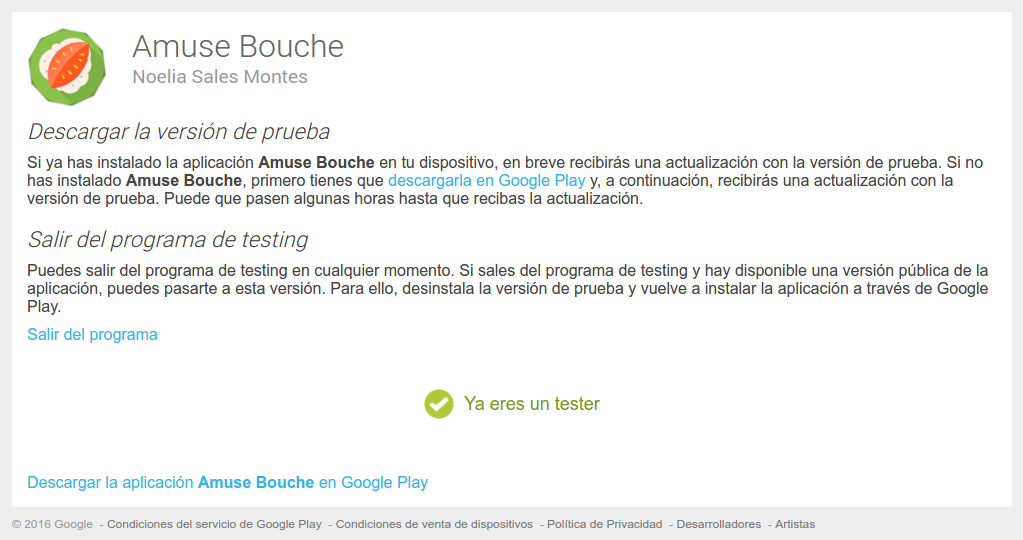
\includegraphics[width=\textwidth]{cap7/img/google-beta}
  \caption{Google Beta}
  \label{fig:google-beta}
\end{figure}


\section{Pruebas funcionales}

\subsection{Pruebas de sistema}


\subsection{Pruebas de aceptación}

\section{Pruebas no funcionales}


\subsection{Pruebas de seguridad}

\subsection{Verificación de la calidad del código}
